\documentclass[../main.tex]{subfiles}

\begin{document}

\section{Probability Theory} \label{probability}
A probability is a measure of how frequent or likely an event will take place. 

\paragraph{Probability Space} \index{Probability Space} The probability space is a triplet space containing a sample/outcome space $\Omega$ (containing all possible atomic events), a collection of events $S$ (containing a subset of $\Omega$ to which we want to assign probabilities) and the mapping $P$ between $\Omega$ and $S$. 
\paragraph{Axioms of Probability} \index{Axioms of Probability} The mapping $P$ must fulfill the axioms of probability: 
        \begin{enumerate}
            \item $P(a) \geq 0$
            \item $P(\Omega) = 1$
            \item $a,b \in S$ and $a \cap b = \{\}$ $ \Rightarrow P(a \cup b) = P(a) + P(b)$
        \end{enumerate}
\paragraph{Random Variable} \index{Random Variable} A random variable is a function that maps points from the sample space $\Omega$ to some range (e.g. Real numbers or booleans). They are characterized by their distribution function. E.g. for a dice roll:
        \[ X(\omega) = \begin{cases} 
            0, \text{ if } \omega = heads\\
            1, \text{ if } \omega = tails.
        \end{cases}
        \]
\paragraph{Proposition} \index{Proposition} A Proposition is a conclusion of a statistical inference that can be true or false (e.g. a classification of a datapoint). More formally: A disjunction of events where the logic model holds. An event can be written as a \textbf{propositional logic model}:\\ $A = true, B = false \Rightarrow a \land \neg b $. Propositions can be continuous, discrete or boolean. 

\subsection{Probability distributions} \index{Probability distribution}
Probability distributions assign probabilities to to all possible points in $\Omega$ (e.g. $P(Weather) = \langle 0.3, 0.4, 0.2, 0.1 \rangle$, representing Rain, sunshine, clouds and snow). 
Joint probability distributions give you a probability for each atomic event of the random variables (e.g. $P(weather, accident)$ gives you a $2\times 4$  matrix.)

\paragraph{Cumulative Distribution Function (CDF)} \index{Cumulative Distribution Function} The CDF is defined as $F_X(x) = P(X \leq x)$ (See figure \ref{CDF}).
        \begin{figure}
            \centering
            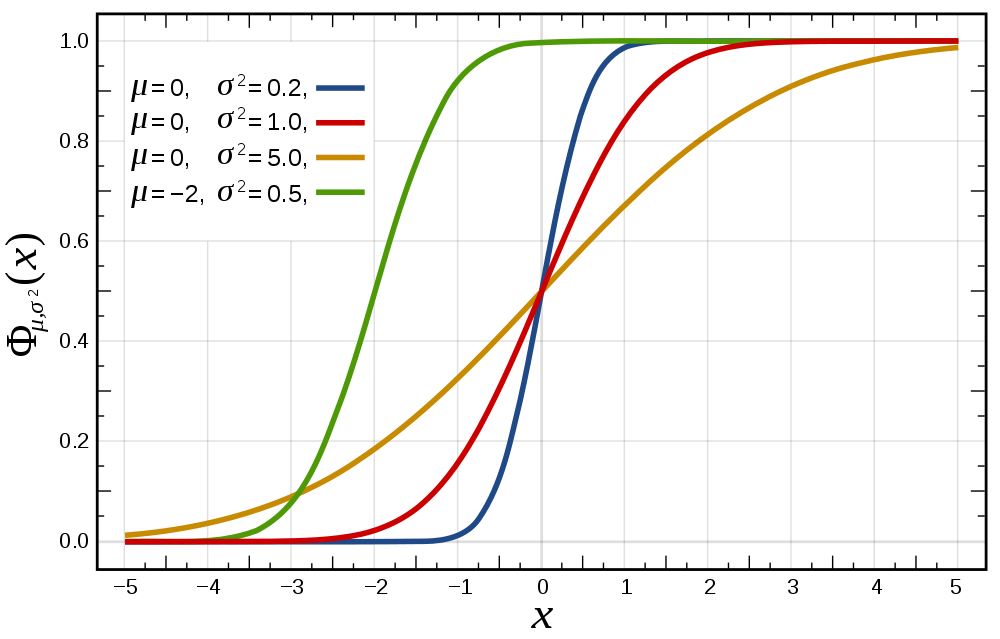
\includegraphics[width=0.6\textwidth]{../figures/Normal_Distribution_CDF.png}
            \caption{Cumulative distribution function of a normal distribution for different mean ($\mu$) and variance ($\sigma$). \textit{Figure from \href{https://commons.wikimedia.org/wiki/File:Normal_Distribution_CDF.svg}{user Inductiveload on wikimedia.org}.}}
            \label{CDF}
        \end{figure}

\paragraph{Probability Density Function (PDF)} \index{{Probability Density Function}} For continuous functions the PDF is defined by 
        \begin{equation}
            p(x) =  {d \over dx} p(X \leq x).
        \end{equation}
        The probability of x being in a finite interval is
        \begin{equation}
            P(a < X \leq b) = \int_a^b p(x) dx
        \end{equation}
        A PDF is shown in figure
        \begin{figure}
            \centering
            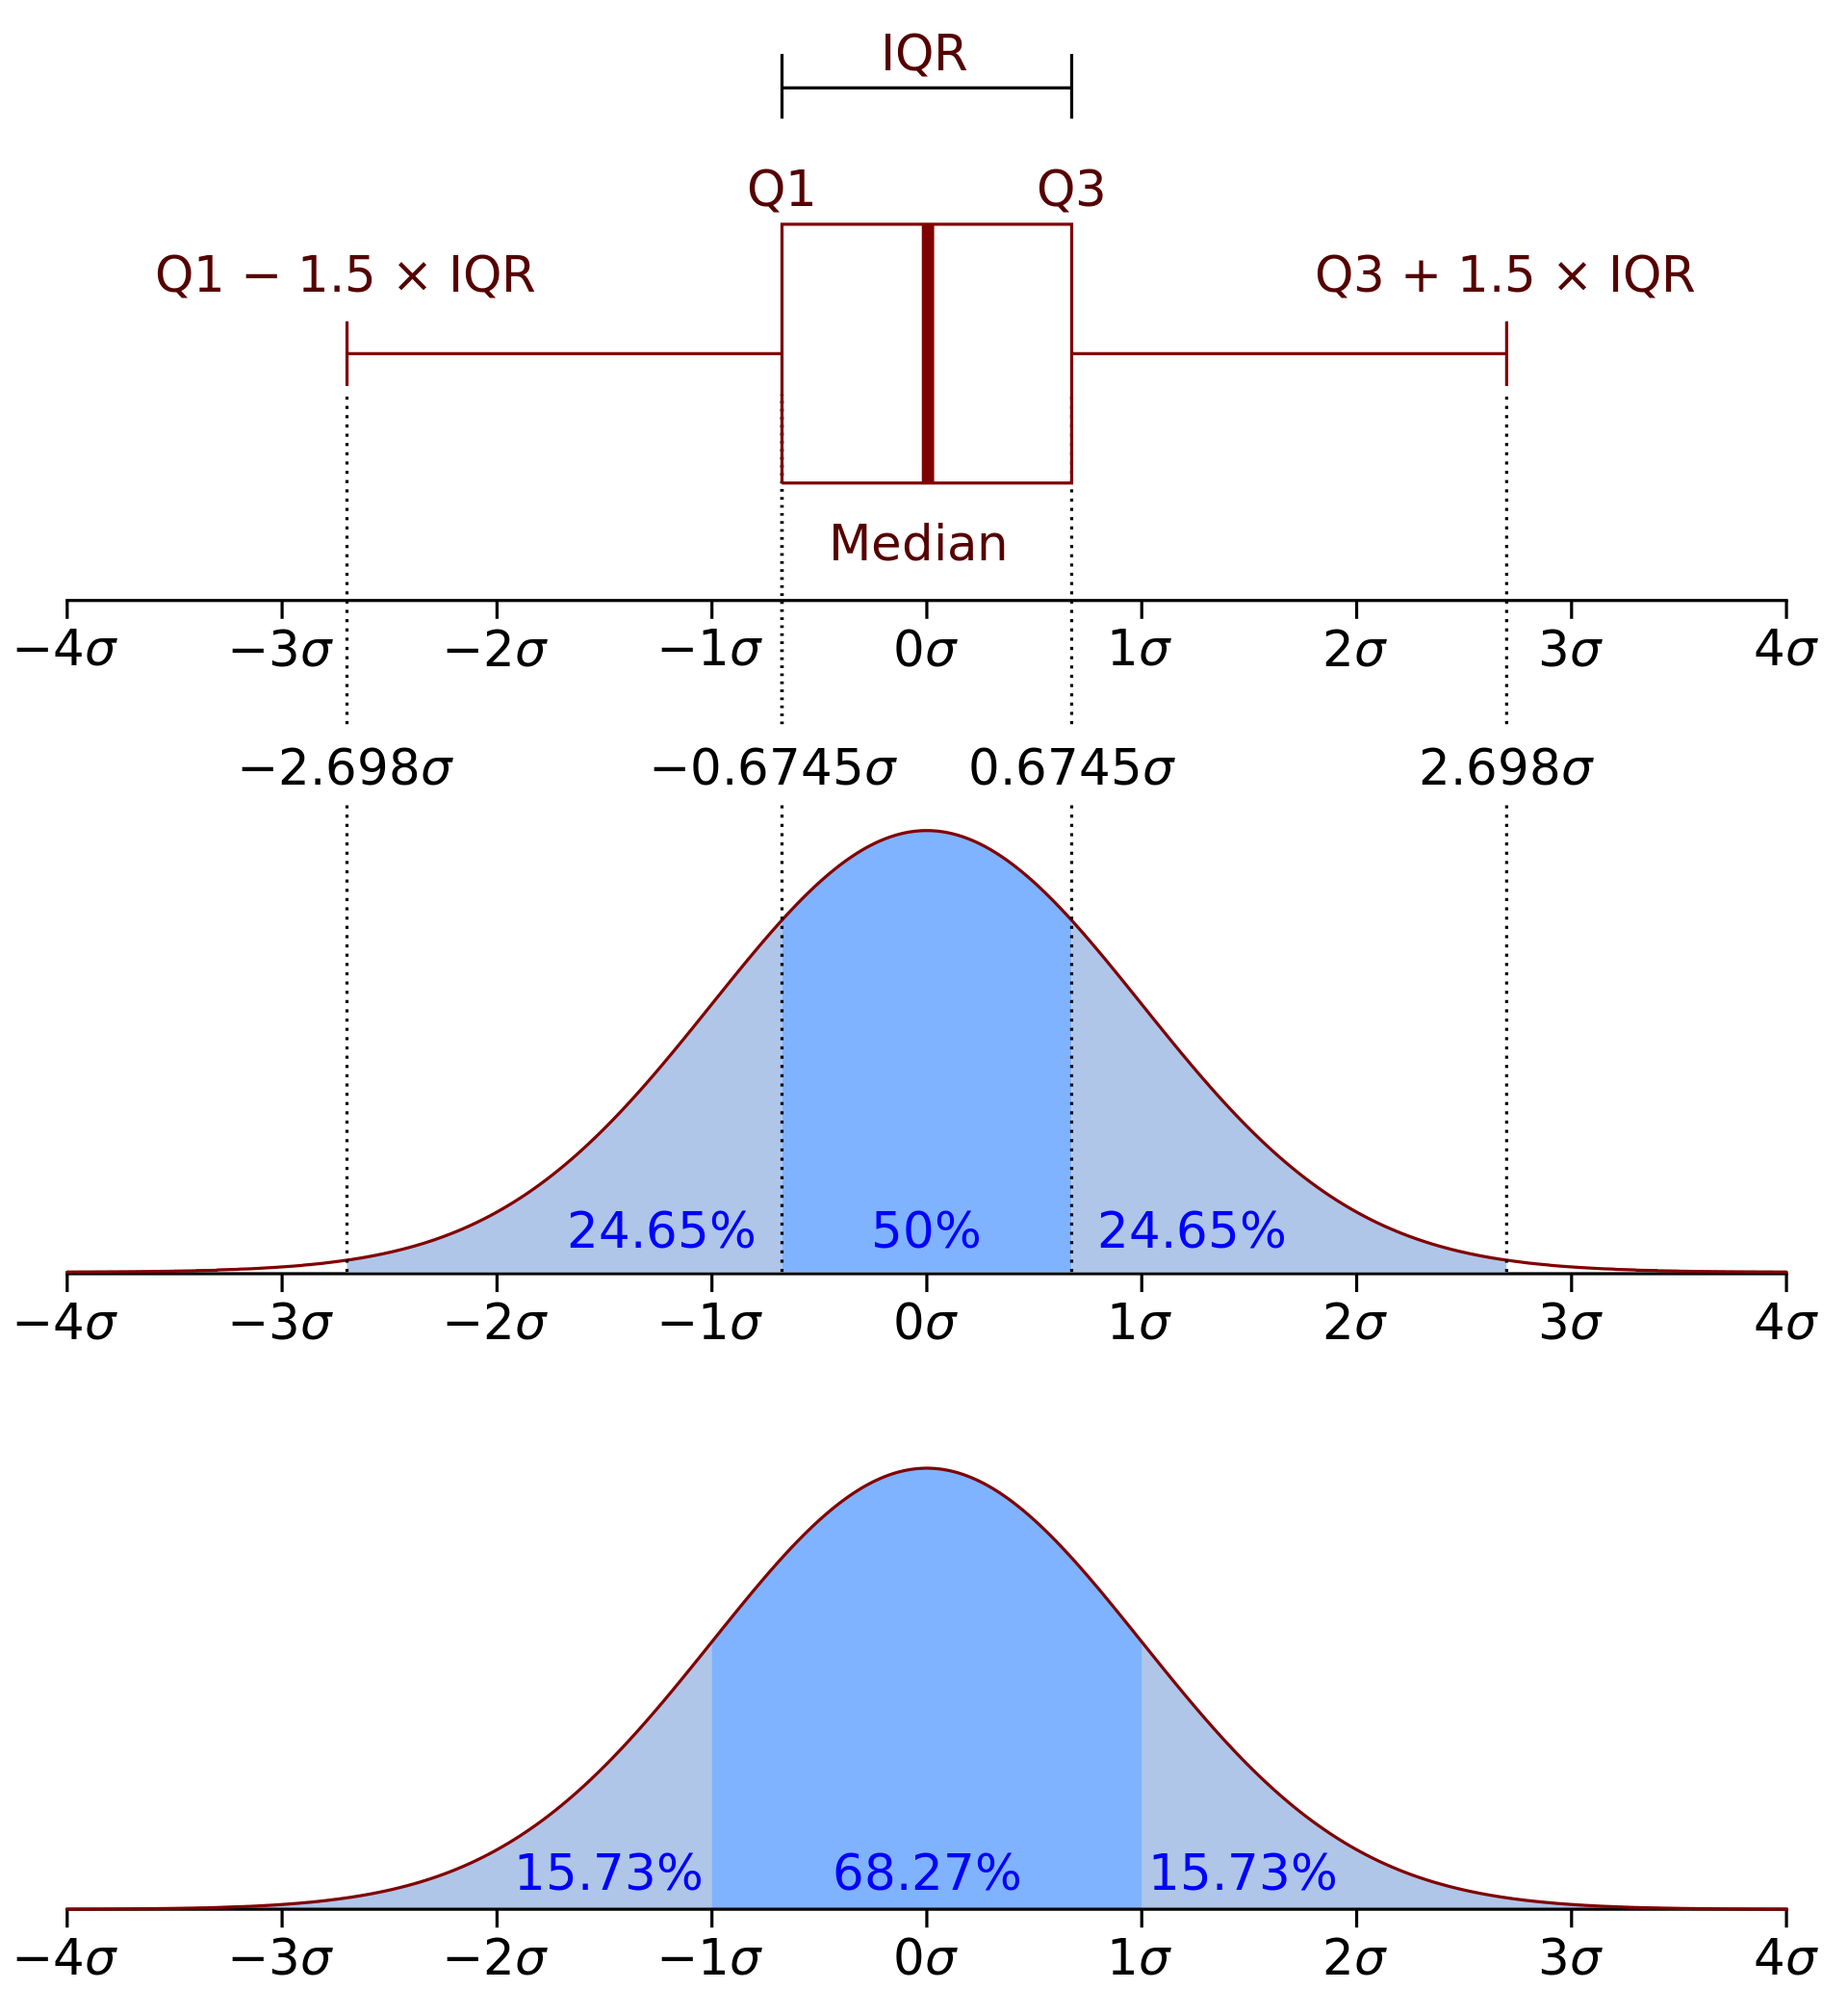
\includegraphics[width=0.6\textwidth]{../figures/Boxplot_vs_PDF.png}
            \caption{Probability density function of a normal distribution with variance ($\sigma$). In red a range from a Box-plot is shown with quartiles (Q1, Q3) and interquartile range (IQR). For the cutoffs (borders to darker blue regions) the IQR (on top) and $\sigma$ are chosen. Another common cutoff is the confidence interval with light blue regions having a probability mass of $2 * \alpha / 2$. \textit{Figure from \href{https://commons.wikimedia.org/wiki/File:Boxplot_vs_PDF.svg}{user Jhguch on wikimedia.org}.}}
            \label{CDF}
        \end{figure}

\paragraph{Uniform distribution} \index{Uniform distribution}
        The uniform distribution has the same probability throughout a specific interval and is defined as 
        % \begin{equation}
        %     \text{Unif}(a,b) = \frac{1}{b-a} \mathbb{I}(a < x \leq b) = 
        % \end{equation}
        \[ \text{Unif}(a,b) = \frac{1}{b-a} \mathbb{I}(a < x \leq b) = \begin{cases} 
            \frac{1}{b-a}, \text{ if } x \in [ a,b ] \\
            0, \text{ else}
        \end{cases}
        \]

\paragraph{Properties of Distributions}


\end{document}
